\documentclass[french]{article}
\usepackage[T1]{fontenc}
\usepackage[utf8]{inputenc}
\usepackage[french]{babel}
\usepackage{amsmath}
\usepackage{mathtools}
\usepackage{color}
\usepackage[svgnames,dvipsnames]{xcolor} 
\usepackage{soul}
\usepackage{amssymb}
\usepackage{enumitem}
\usepackage{multicol}
\usepackage[left=2cm,right=2cm,top=2cm,bottom=2cm]{geometry}
\newcommand{\mathcolorbox}[2]{\colorbox{#1}{$\displaystyle #2$}}
\usepackage{pifont}
\usepackage{pst-all}
\usepackage{pstricks}
\usepackage{delarray}
\usepackage{setspace}
\usepackage{graphicx}
\usepackage{hyperref}
\usepackage{nicematrix}
\usepackage{listings}
\usepackage{float}

% pour l'indicatrice
\usepackage{bbold}


\hypersetup{
	colorlinks=true,
	linkcolor=blue,
	filecolor=magenta,      
	urlcolor=cyan,
	pdfpagemode=FullScreen,
}

\usepackage{amsthm}
\newtheorem*{Rem}{Remarque}

\newenvironment{conclusion}[1]{%
	\begin{center}\normalfont\textbf{Conclusion}\end{center}
	\begin{quotation} #1 \end{quotation}
}{%
	\vspace{1cm}
}

\newcommand\pythonstyle{\lstset{
	language=Python,
	basicstyle=\ttm,
	morekeywords={self},              % Add keywords here
	keywordstyle=\ttb\color{deepblue},
	emph={MyClass,__init__},          % Custom highlighting
	emphstyle=\ttb\color{deepred},    % Custom highlighting style
	stringstyle=\color{deepgreen},
	frame=tb,                         % Any extra options here
	showstringspaces=false
}}

\lstdefinestyle{Cpp}{
	language=C++,
	tabsize=3,
	basicstyle=\ttfamily,
	keywordstyle=\color{blue}\ttfamily,
	stringstyle=\color{red}\ttfamily,
	commentstyle=\color{green}\ttfamily,
	morecomment=[l][\color{magenta}]{\#}
}

\lstdefinestyle{Python}{
	language=Python,
	tabsize=3,
	basicstyle=\ttfamily,
	keywordstyle=\color{blue}\ttfamily,
	stringstyle=\color{red}\ttfamily,
	commentstyle=\color{green}\ttfamily,
	morecomment=[l][\color{magenta}]{\#}
}

\lstset{style=Cpp}

\setlength\parindent{0pt}


\usepackage{fontawesome}

\usepackage{lipsum}

% overline \hl{...}
\usepackage{soul}
% recall box
\usepackage[most]{tcolorbox}

% \begin{preuve} ... \end{preuve}

\newenvironment{preuve}[1][]{\begin{tcolorbox}[
	colback=white, % Couleur de fond de la boîte
	colframe=green!70!black, % Couleur du cadre de la boîte
	arc=2mm, % Rayon de l'arrondi des coins
	boxrule=1pt, % Épaisseur du cadre de la boîte
	breakable, enhanced jigsaw
	]
	\textcolor{green!70!black}{\textbf{Preuve.} \\}

	#1
}{\end{tcolorbox}}

% \begin{rappel} ... \end{rappel}

\newenvironment{rappel}[1][]{\begin{tcolorbox}[
	colback=white, % Couleur de fond de la boîte
	colframe=blue!70!black, % Couleur du cadre de la boîte
	arc=2mm, % Rayon de l'arrondi des coins
	boxrule=1pt, % Épaisseur du cadre de la boîte
	breakable, enhanced jigsaw
	]
	\textcolor{blue!70!black}{\textbf{Rappel.} \\}

	#1
}{\end{tcolorbox}}

\newenvironment{remarque}[1][]{\begin{tcolorbox}[
	colback=white, % Couleur de fond de la boîte
	%colframe=black!70!black, % Couleur du cadre de la boîte
	arc=2mm, % Rayon de l'arrondi des coins
	%boxrule=0.5pt, % Épaisseur du cadre de la boîte
	borderline={0.5mm}{0mm}{black!15!white},
	borderline={0.5mm}{0mm}{black!50!white,dashed},
	breakable, enhanced jigsaw
	]
	\textcolor{black!70!black}{\textbf{Remarque.}} #1
}{\end{tcolorbox}}

% \sethlcolor{lightblue}

\begin{document}
	LECOURTIER Frédérique \hfill \today
	\begin{center}
		\Large\textbf{{PINNs et Méthodes numériques}}
	\end{center}

	\section{Introduction}

    On considère une équation elliptique de la forme
    \begin{equation}
		\left\{\begin{aligned}
			&L(u)=-\nabla \cdot (A(x) \nabla u(x)) + c(x)u(x) = f(x) \quad \text{dans } \Omega \\
			&u(x) = g(x) \quad \text{sur } \partial \Omega
		\end{aligned}\right. \label{edp}
	\end{equation}

	\textbf{Formulation faible :} 
	
	On multiplie par une fonction test $v$ et on intègre par parties pour obtenir

	\begin{equation}
		a(u,v)=l(v)
	\end{equation}

	avec

	\begin{align*}
		a(u,v)&=\int_{\Omega} (A(x)\nabla u(x)) \cdot \nabla v(x) + c(x)u(x)v(x) \, dx \\
		l(v)&=\int_{\Omega} f(x)v(x) \, dx
	\end{align*}

	% \int_{\Omega} (A(x)\nabla u(x)) \cdot \nabla v(x) + c(x)u(x)vv \, dx = \int_{\Omega} f(x)v(x) \, dx

	\textbf{Existence et unicité :} Lax-Milgram

	\hl{A compléter !}

	\textbf{Problème de minimsation équivalent :} 
	
	Comme $a$ est symétrique, le théorème de Lax-Milgram implique le problème de minimisation suivant équivalent :

	\begin{equation}
		u(x)=\arg\min_{v \in V}J(v) \label{min}
	\end{equation}

	avec
	\begin{align*}
		J(v)&=\frac{1}{2}a(v,v) - l(v) \\
		&=\frac{1}{2} \int_{\Omega} L(v) v - \int_{\Omega} fv \\
		&=\frac{1}{2} \int_{\Omega} (A\nabla v) \cdot \nabla v + cv^2 - \int_{\Omega} fv
	\end{align*}

	On considère un problème en dimension infinie puisqu'on cherche une fonction. L'enjeu des méthodes numériques est de discrétiser ce problème et de le résoudre dans un espace de dimension finie. La résolution se décomposer alors en les étapes suivantes :
	\begin{enumerate}[label=\textbullet]
		\item \textbf{Encodage :} on encode le problème dans un espace de dimension finie
		\item \textbf{Approximation :} on résout le problème dans l'espace de dimension finie
		\item \textbf{Décodage :} on ramène la solution dans l'espace de dimension infinie
	\end{enumerate}

	\begin{center}
		\begin{tabular}{|c|c|c|}
			\hline
			\textbf{Encodeur} & \textbf{Approximateur} & \textbf{Décodeur} \\
			\hline
			$f \; \rightarrow \theta_f$ & $\theta_f \; \rightarrow \theta_u$ & $\theta_u \; \rightarrow u_\theta$ \\
			\hline
		\end{tabular}
	\end{center}

	\section{Méthodes Eléments Finis Standard}

	\subsection{Encodeur/Décodeur}

	En pratique, on commence par définir le décodeur car c'est lui qui va nous fournir l'espace de dimension finie dans lequel on va travailler. On définit ensuite l'encodeur et l'approximateur en fonction de l'espace de dimension finie choisi.

	\begin{enumerate}[label=\textbullet]
		\item \textbf{Décodeur :} Dans le cadre des méthodes éléments finis, on choisit un espace de dimension finie $V_N$ de fonctions polynomiales par morceaux $\{\varphi_i\}_{i=1}^N$. On définit alors le décodeur comme la combinaison linéaire de ces fonctions de base :
		\begin{equation*}
			D_\theta(x) = \sum_{i=1}^N \theta_i \varphi_i(x)
		\end{equation*}
		\item \textbf{Encodeur :} Comme l'espace $V_N$ est un espace vectoriel, il existe une définition naturelle de l'encodeur qui consiste à considérer le projecteur orthogonal sur $V_N$ :
		\begin{equation*}
			\theta_f = E(f) = M^{-1} b(f)
		\end{equation*}
		avec 
		\begin{align*}
			M_{ij} &= \langle \varphi_i, \varphi_j\rangle = \int_{\Omega} \varphi_i(x) \varphi_j(x) \, dx \\
			b_i(f) &= \langle f, \varphi_i \rangle = \int_{\Omega} f(x) \varphi_i(x) \, dx
		\end{align*}
		
		\begin{rappel}			
			\begin{minipage}{0.3\linewidth}
				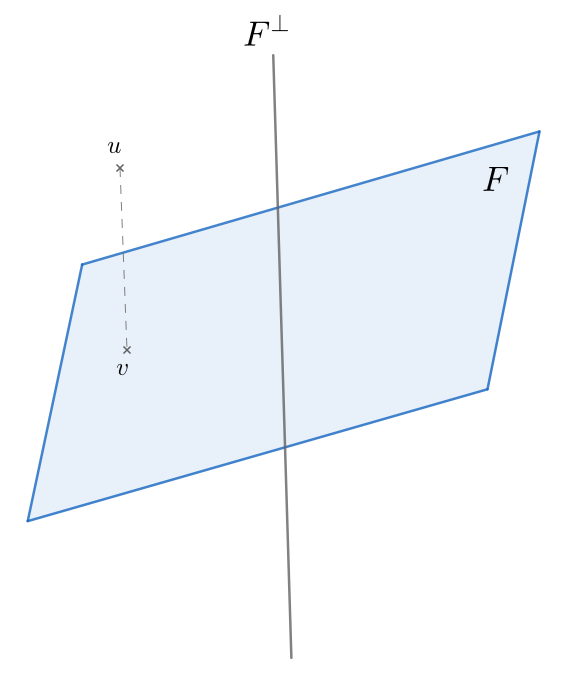
\includegraphics[width=\linewidth]{images/ortho.png}
			\end{minipage} \qquad 
			\begin{minipage}{0.6\linewidth}
				\textbf{Projection orthogonale :}
				$$v = p_F(u) \quad \iff \quad \left\{\begin{aligned}
					&v\in F \\
					&u-v\in F^\perp
				\end{aligned}\right.$$

				Si $F=Vect\{e_1,\dots,e_n\}$, alors
				$$u\in F^\perp \quad \iff \quad \forall i\in\{1,\dots,k\}, \quad \langle u,e_i\rangle=0$$
			\end{minipage}
		\end{rappel}

		\begin{preuve}			
			Ainsi, on souhaite projeter $f$ sur le sous-espace vectoriel $V_N$ de sorte à ce que
			
			\begin{equation*}
				f_\theta = p_{V_N}(f)
			\end{equation*}
			
			alors $\forall i \in \{1,\dots,N\}$, on a
			
			\begin{align*}
				&\quad \langle f_\theta - f, \varphi_i \rangle = 0 \\
				\iff &\quad \langle f_\theta, \varphi_i \rangle = \langle f, \varphi_i \rangle \quad  \\
				\iff &\quad \sum_{j=1}^N(\theta_f)_j \langle \varphi_j, \varphi_i\rangle = \langle f, \varphi_i \rangle \\ 
				\iff &\quad M \theta_f = b(f) \\
				\iff &\quad \theta_f = M^{-1} b(f)
			\end{align*}
			
			avec 
			
			\begin{align*}
				M_{ij} &= \langle \varphi_i, \varphi_j\rangle = \int_{\Omega} \varphi_i(x) \varphi_j(x) \, dx \\
				b_i(f) &= \langle f, \varphi_i \rangle = \int_{\Omega} f(x) \varphi_i(x) \, dx
			\end{align*}
			
		\end{preuve}
	\end{enumerate}
	
	\subsection{Approximateur}
	
	La stratégie utilisée précédemment consiste à faire une projection d’une certaine forme de l’équation sur l’espace de dimension finis $V_N$. Par unicité de la projection orthogonale on va donc se ramener à un problème sur les degrés de liberté qui lui aussi aura une unique solution. Par contre, on peut obtenir plusieurs variantes pour chaque méthode selon la forme du problème qu’on utilise pour la projection. On va introduire deux projections (Galerkin et Galerkin moindre carrés) et montrer à quel problème sur les degrés de liberté elles se ramènent.
	
	\subsubsection{Projection de Galerkin}
			
	\begin{itemize}[label=\ding{222}]
		\item \textbf{Problème de minimisation considéré :}
		
		Dans ce cas, on considère en fait le même problème de minimisation que celui défini par \eqref{min}. Pour l'unicité du problème, on va considérer un résidu qui inclut les conditions au bord (condition de Dirichlet). On définit alors le résidu par
		
		\begin{equation*}
			R(v) = R_i(v)\mathbb{1}_{\Omega} + R_{bc}(v)\mathbb{1}_{\partial \Omega}
		\end{equation*}
	
		avec 
		
		\begin{equation*}
			R_i(v)=L(v) - f \qquad \text{et} \qquad R_{bc}(v)=v-g
		\end{equation*}
		
		qui définissent respectivement les résidus à l'intérieur de $\Omega$ et sur le bord $\partial\Omega$. 
		
		Ainsi on peut définir le problème à minimiser par

		\begin{equation}
			u(x)=\arg\min_{v \in V}J(v) \label{min_galerkin}
		\end{equation}
	
		où
		\begin{equation*}
			J(v)=J_i(v)+J_{bc}(v) 
		\end{equation*}
		
		avec 
		
		\begin{equation*}
			J_i(v)=\frac{1}{2}\int_\Omega L(v)v - \int_\Omega fv  \qquad \text{et} \qquad J_{bc}(v)=\frac{1}{2}\int_\Omega R_{bc}(v)^2
		\end{equation*}

		On peut vérifier que la résolution du problème de minimisation \eqref{min_galerkin} est équivalent à la résolution de l'EDP \eqref{edp}.
		
		\begin{preuve}
			On suppose ici que $J$ est différentiable \hl{A faire ?}. Calculons alors sa différentielle :
			
			\begin{itemize}[label=\textbullet]
				\item Calculons dans un premier la différentielle de $J_{i}$ :
				\begin{align*}
					J_i(v+\epsilon h)=\frac{1}{2} \int_{\Omega} (A\nabla(v+\epsilon h)) \cdot \nabla(v+\epsilon h) + c(v+\epsilon h)^2 - \int_{\Omega} f(v+\epsilon h)
				\end{align*}
	
				Or par bilinéarité du produit scalaire et par symétrie de $A$, on a
				\begin{align*}
					(A\nabla(v+\epsilon h)) \cdot \nabla(v+\epsilon h) &= (A\nabla v) \cdot \nabla v + \epsilon (A\nabla v) \cdot \nabla h + \epsilon (A\nabla h) \cdot \nabla v + \epsilon^2 (A\nabla h) \cdot \nabla h \\
					&= (A\nabla v) \cdot \nabla v + 2\epsilon (A\nabla v) \cdot \nabla h + \epsilon^2 (A\nabla h) \cdot \nabla h \\
				\end{align*}
	
				donc
				\begin{align*}
					\frac{J_i(v+\epsilon h)-J_i(v)}{\epsilon} = \int_{\Omega} (A\nabla v) \cdot \nabla h + \frac{\epsilon}{2} (A\nabla h) \cdot \nabla h + cvh+ \frac{\epsilon}{2}ch^2 - fh
				\end{align*}
	
				On en déduit que
				\begin{align*}
					\mathcal{D}J_i(v)\cdot h &= \int_{\Omega} (A\nabla v) \cdot \nabla h + cvh - fh \\
					&= \int_{\Omega} (-\nabla\cdot(A\nabla v) + cv - f)h \\
				\end{align*}
	
				Et finalement on en déduit que le gradient de $J_i$ est égal au résidu de l'équation de départ :
				\begin{align*}
					\nabla_v J_i(v) &= -\nabla\cdot(A\nabla v) + cv - f \\
					&= L(v) - f = R_i(v)
				\end{align*}
			
				\item De la même manière, on peut calculer la différentielle de $J_{bc}$ :
				\begin{align*}
					J_{bc}(v+\epsilon h)=\frac{1}{2} \int_{\Omega} v^2+2\epsilon vh +\epsilon^2 h^2 - 2vg - 2\epsilon hg+g^2
				\end{align*}

				donc
				\begin{align*}
					\frac{J_{bc}(v+\epsilon h)-J_{bc}(v)}{\epsilon} = \int_{\Omega} v^2+\frac{\epsilon}{2} h^2 - hg
				\end{align*}
				
				On en déduit que
				\begin{align*}
					\mathcal{D}J_{bc}(v)\cdot h = \int_{\Omega} v^2 - hg
				\end{align*}
				
				Et finalement on en déduit le gradient de $J_{bc}$ :
				\begin{align*}
					\nabla_v J_{bc}(v) = (v-g) = R_{bc}(v) 
				\end{align*}
			\end{itemize}
		
			Finalement
			\begin{equation*}
				\nabla_v J(v) = \nabla_v  J_{i}(v) + \nabla_v J_{bc}(v) = R(v)
			\end{equation*}
		
			Ainsi $u_\theta$ est solution du problème de minimisation implique
			\begin{equation*}
				\nabla_v J(u_\theta)=0 \quad \Rightarrow \quad \left\{\begin{aligned}
					&R(u_\theta)=0 \quad \Omega \\
					&u_\theta=g \quad \partial\Omega
				\end{aligned}\right.
			\end{equation*}
			et $u_\theta$ vérifie bien l'équation \eqref{edp}.
		\end{preuve}
		
		\item \textbf{Résolution numérique :}
		
		La projection de Galerkin consiste à projeter l'EDP sur l'espace $V_N$ de sorte à ce que $\forall v \in V_N$ :
		
		\begin{equation*}
			\langle R(u_\theta(x)), v\rangle_{L^2} = 0
		\end{equation*}
		
		avec $R$ le résidu de l'équation défini par :
		
		\begin{equation*}
			R(v) = L(v) - f
		\end{equation*}
		
		On cherche à montrer ici que la projection de Galerkin est équivalente à la minimisation de $J$ sur $V_N$. Plus précisément, comme dans le cadre de la méthode des éléments finis, on a construit une base de $V_N$ à partir de fonctions de base polynomiale $\{\varphi_i\}_{i=1}^N$, on peut écrire la projection de Galerkin sous la forme suivante :

		\begin{equation*}
			\langle R(u_\theta(x)), \varphi_i\rangle_{L^2} = 0 \quad \forall i \in \{1,\dots,N\}
		\end{equation*}

		et le problème de minimisation s'écrit sous la forme d'un problème discret :
		
		\begin{equation}
			\theta_u = \arg\min_{\theta \in \mathbb{R}^N}J(\theta) \label{min_galerkin_discret}
		\end{equation}
		
		avec
		\begin{equation*}
			J(\theta)=\frac{1}{2}\int_\Omega L(v_\theta)v_\theta - \int_\Omega fv_\theta
		\end{equation*}
	
		\begin{remarque}
			On peut remarquer ici que le problème de minimisation définit ici n'inclue pas explicitement les conditions de bord. Dans la pratique, on utilise deux types de méthodes pour imposer les conditions au bord soit par pénalisation soit en le incluant directement dans les fonctions de bases. De ce fait, ici on ne va s'intéresser qu'au problème sur $\Omega$ sans tenir compte des conditions de bord.
		\end{remarque}
	
		\begin{preuve}			
			On suppose ici que $J$ est différentiable \hl{A faire ?}. Calculons alors sa différentielle par rapport à $\theta$.
			
			On commence par définir 
			\begin{equation*}
				v_\theta=\sum_{i=1}^{N} \theta_i \varphi_i=\theta\cdot\varphi \qquad \text{et} \qquad v_{\theta+\epsilon h}=(\theta+\epsilon h)\cdot\varphi=v_\theta+\epsilon v_h
			\end{equation*}
		
			alors comme $A$ est symétrique

			\begin{align*}
				J(\theta+\epsilon h)&=\frac{1}{2} \int_{\Omega} (A\nabla(v_{\theta+\epsilon h})) \cdot \nabla(v_{\theta+\epsilon h}) + c(v_{\theta+\epsilon h})^2 - \int_{\Omega} fv_{\theta+\epsilon h} \\
				&=\frac{1}{2} \int_{\Omega} (A\nabla v_\theta) \cdot \nabla v_\theta + 2\epsilon (A\nabla v_\theta) \cdot \nabla v_h + \epsilon^2 (A\nabla v_h) \cdot \nabla v_h + cv_\theta^2+2\epsilon cv_\theta v_h \\
				& \qquad +\epsilon^2cv_h^2 - \int_{\Omega} fv_\theta+\epsilon fv_h
			\end{align*}
			
			Finalement
			\begin{align*}
				\frac{J(\theta+\epsilon h)-J(\theta)}{\epsilon} = \int_{\Omega} (A\nabla v_\theta) \cdot \nabla v_h + \frac{\epsilon}{2} (A\nabla v_ h) \cdot \nabla v_h + cv_\theta v_h+ \frac{\epsilon}{2}cv_h^2 - fv_h
			\end{align*}
			
			et
			\begin{align*}
				\mathcal{D}J(\theta)\cdot h &= \int_{\Omega} (A\nabla v_\theta) \cdot \nabla v_h + cv_\theta v_h - fv_h \\
				&=\int_\Omega R(v_\theta)v_h \\
				&=\sum_{i=1}^N h_i\int_\Omega R(v_\theta)\varphi_i
			\end{align*}
			
			Ainsi le gradient de $J$ par rapport à $\theta$ est défini par :
			\begin{align*}
				\nabla_\theta J(\theta) = \left(\int_\Omega R(v_\theta)\varphi_i\right)_{i=1,\dots,N}
			\end{align*}
			
			On en déduit alors que résoudre le problème de minimisation \eqref{min_galerkin_discret} revient à effectuer la projection de Galerkin définie par
			\begin{equation*}
				\langle R(u_\theta(x)), \varphi_i\rangle_{L^2} = 0 \quad \forall i \in \{1,\dots,N\}
			\end{equation*}
		\end{preuve}
	\end{itemize}		
	
	\subsubsection{Projection de Galerkin moindre-carré :}
	
	\begin{itemize}[label=\ding{222}]
		\item \textbf{Problème de minimisation considéré :}
		
		On considère maintenant le problème de minimisation moindre-carré en considérant un résidu qui inclut les conditions au bord (condition de Dirichlet). On définit alors le résidu de la même manière que précédemment :
		\begin{equation*}
			R(v) = R_i(v)\mathbb{1}_{\Omega} + R_{bc}(v)\mathbb{1}_{\partial \Omega}
		\end{equation*}
		
		avec 
		
		\begin{equation*}
			R_i(v)=L(v) - f \qquad \text{et} \qquad R_{bc}(v)=v-g
		\end{equation*}
		
		qui définissent respectivement les résidus à l'intérieur de $\Omega$ et sur le bord $\partial\Omega$. 
		
		On peut alors définir le problème moindre-carré de la façon suivante
		
		\begin{equation}
			u(x)=\arg\min_{v \in V}J(v) \label{min_moindrecarre}
		\end{equation}
		
		où
		\begin{equation*}
			J(v)=J_i(v)+J_{bc}(v) 
		\end{equation*}
		
		avec 
		
		\begin{equation*}
			J_i(v)=\frac{1}{2}\int_\Omega R_i(v)^2  \qquad \text{et} \qquad J_{bc}(v)=\frac{1}{2}\int_\Omega R_{bc}(v)^2
		\end{equation*}
		
		On peut vérifier que la résolution du problème de minimisation \eqref{min_moindrecarre} est équivalent à la résolution de l'EDP \eqref{edp}.
		
		\begin{remarque}
			A noter que $J_{bc}$ est identique que dans le cas de la projection par Galerkin.
		\end{remarque}
		
		\begin{preuve}
			On suppose ici que $J$ est différentiable \hl{A faire ?}. Calculons alors sa différentielle :
			
			\begin{itemize}[label=\textbullet]
				\item Calculons dans un premier la différentielle de $J_{i}$. Notons que
				\begin{align*}
					J_i(v) &= \frac{1}{2} \int_{\Omega} (L(v) - f)^2=\frac{1}{2} \int_{\Omega} R(v)^2 \\
					&= \frac{1}{2}\langle R(v), R(v) \rangle_{L^2} \\
					&= \frac{1}{2}\langle -\nabla\cdot(A\nabla v) + cv - f, -\nabla\cdot(A\nabla v) + cv - f \rangle_{L^2} \\
					&= \frac{1}{2}\left[\langle \nabla\cdot(A\nabla v), \nabla\cdot(A\nabla v) \rangle_{L^2} -2 \langle \nabla\cdot(A\nabla v), cv \rangle_{L^2} +2 \langle \nabla\cdot(A\nabla v), f \rangle_{L^2} + \langle cv, cv \rangle_{L^2}\right. \\
					& \qquad \qquad \left.-2 \langle cv,f\rangle_{L^2} + \langle f, f \rangle_{L^2}\right]
				\end{align*}

				Ainsi
				\begin{align*}
					J_i(v+\epsilon h)&= \frac{1}{2}\left[\langle \nabla\cdot(A\nabla (v+\epsilon h)), \nabla\cdot(A\nabla (v+\epsilon h)) \rangle_{L^2} -2 \langle \nabla\cdot(A\nabla (v+\epsilon h)), c(v+\epsilon h) \rangle_{L^2}\right. \\
					& \qquad \left. + 2 \langle \nabla\cdot(A\nabla (v+\epsilon h)), f \rangle_{L^2} + \langle c(v+\epsilon h), c(v+\epsilon h) \rangle_{L^2} -2 \langle c(v+\epsilon h),f\rangle_{L^2} + \langle f, f \rangle_{L^2}\right] \\
					&= \frac{1}{2}\left[\langle \nabla\cdot(A\nabla v), \nabla\cdot(A\nabla v) \rangle +2\epsilon\langle \nabla\cdot(A\nabla v), \nabla\cdot(A\nabla h) \rangle +\epsilon^2\langle \nabla\cdot(A\nabla h), \nabla\cdot(A\nabla h) \rangle\right. \\
					& \quad \left.-2 \langle \nabla\cdot(A\nabla v), cv \rangle-2\epsilon \langle \nabla\cdot(A\nabla v), ch \rangle-2\epsilon \langle \nabla\cdot(A\nabla h), cv \rangle-\epsilon^2 \langle \nabla\cdot(A\nabla h), ch \rangle\right. \\
					& \quad \left. + 2 \langle \nabla\cdot(A\nabla v), f \rangle+ 2\epsilon \langle \nabla\cdot(A\nabla h), f \rangle \right. \\
					& \quad \left. + \langle cv, cv \rangle+2\epsilon \langle cv, ch \rangle + \epsilon^2 \langle ch, ch \rangle -2 \langle cv,f\rangle-2\epsilon \langle ch,f\rangle + \langle f, f \rangle\right]
				\end{align*}
	
				donc
	
				\begin{align*}
					\frac{J_i(v+\epsilon h)-J_i(v)}{\epsilon}&= \langle \nabla\cdot(A\nabla v), \nabla\cdot(A\nabla h) \rangle-\langle \nabla\cdot(A\nabla v), ch \rangle-\langle \nabla\cdot(A\nabla h), cv \rangle \\ 
					& \quad +\langle \nabla\cdot(A\nabla h), f \rangle + \langle cv, ch \rangle -\langle ch,f\rangle \\
					& \quad + \frac{\epsilon}{2}\left[\langle \nabla\cdot(A\nabla h), \nabla\cdot(A\nabla h) \rangle-\langle \nabla\cdot(A\nabla h), ch \rangle+ \langle ch, ch \rangle \right]
				\end{align*}
	
				On en déduit que
	
				\begin{align*}
					\mathcal{D}J_i(v)\cdot h &= \langle \nabla\cdot(A\nabla h), \nabla\cdot(A\nabla v) - cv +f \rangle+\langle ch, -\nabla\cdot(A\nabla v) + cv - f \rangle \\ 
					&= -\langle \nabla\cdot(A\nabla h), R_i(v) \rangle+\langle ch, R_i(v)\rangle \\ 
					&= \langle -\nabla\cdot(A\nabla R_i(v))+cR_i(v), h \rangle \\
					&= \langle L(R_i(v)), h \rangle \\
				\end{align*}
	
				car par IPP (et comme $A$ symétrique), on a
	
				\begin{align*}
					\langle \nabla\cdot(A\nabla h), R_i(v) \rangle_{L^2}&=\int_{\Omega} \nabla\cdot(A\nabla h)\times R_i(v) \\
					&=-\int_{\Omega} (A\nabla h)\cdot\nabla R_i(v) \\
					&=-\int_{\Omega} \nabla h\cdot(A\nabla R_i(v)) \\
					&=\int_{\Omega} h\times\nabla\cdot(A\nabla R_i(v)) \\
				\end{align*}
	
	
				Et finalement on en déduit que le gradient de $J_i$ par rapport à $v$ est défini par :
	
				\begin{align*}
					\nabla_v J_i(v) &= L(R_i(v)) \\
				\end{align*}
			
				\item De la même manière, on peut calculer la différentielle de $J_{bc}$ :
				\begin{align*}
					J_{bc}(v+\epsilon h)=\frac{1}{2} \int_{\Omega} v^2+2\epsilon vh +\epsilon^2 h^2 - 2vg - 2\epsilon hg+g^2
				\end{align*}
				
				donc
				\begin{align*}
					\frac{J_{bv}(v+\epsilon h)-J_{bc}(v)}{\epsilon} = \int_{\Omega} v^2+\frac{\epsilon}{2} h^2 - hg
				\end{align*}
				
				On en déduit que
				\begin{align*}
					\mathcal{D}J_{bc}(v)\cdot h = \int_{\Omega} v^2 - hg
				\end{align*}
				
				Et finalement on en déduit le gradient de $J_{bc}$ :
				\begin{align*}
					\nabla_v J_{bc}(v) = (v-g) = R_{bc}(v) 
				\end{align*}
			\end{itemize}
		
			\hl{A discuter !}
		
			Finalement
			\begin{align*}
			\nabla_v J(v) &= \nabla_v  J_{i}(v) + \nabla_v J_{bc}(v) \\
			&= L(R(v))\mathbb{1}_\Omega + (v-g)\mathbb{1}_{\partial\Omega}
			\end{align*}
			
			Ainsi $u_\theta$ est solution du problème de minimisation implique
			\begin{equation*}
			\nabla_v J(u_\theta)=0 \quad \Rightarrow \quad \left\{\begin{aligned}
				&L(R(u_\theta))=0 \quad \Omega \\
				&u_\theta=g \quad \partial\Omega
			\end{aligned}\right. \quad \Rightarrow \quad \left\{\begin{aligned}
				&L(R(u_\theta))=0 \quad \Omega \\
				&R(u_\theta)=0 \quad \partial\Omega
			\end{aligned}\right.
			\end{equation*}
		
			Ainsi $R(u_\theta)=0$ partout et $u_\theta$ vérifie bien l'équation \eqref{edp}.
		\end{preuve}

		\item \textbf{Résolution numérique :}
		
		La projection de Galerkin moindre carré consiste à projeter l'EDP sur l'espace $W_N=Vect(\nabla_\theta R(u_\theta(x)))$ de sorte à ce que :
		
		\begin{equation*}
			\langle R(u_\theta(x)), (\nabla_\theta R(u_\theta(x)))_i\rangle_{L^2} = 0, \quad \forall i \in \{1,\dots,N\}
		\end{equation*}
		
		avec $R$ le résidu de l'équation défini par :
		
		\begin{equation*}
			R(v) = L(v) - f
		\end{equation*}
		
		On cherche à montrer ici que la projection de Galerkin moindre-carré est équivalente au problème de minimisation moindre-carré défini précédemment. Plus précisément, le problème de minimisation s'écrit sous la forme d'un problème discret :
		
		\begin{equation}
			\theta_u = \arg\min_{\theta \in \mathbb{R}^N}J(\theta) \label{min_moindrecarre_discret}
		\end{equation}
		
		avec
		\begin{equation*}
			J(\theta)=\frac{1}{2}\int_\Omega R(v_\theta)^2
		\end{equation*}
		
		\begin{remarque}
			De la même manière, on ne s'intéresse pas aux conditions de bord ici.
		\end{remarque}
	
		\begin{preuve}			
			On suppose ici que $J$ est différentiable \hl{A faire ?}. Calculons alors sa différentielle par rapport à $\theta$.
			
			On commence par définir 
			\begin{equation*}
				v_\theta=\sum_{i=1}^{N} \theta_i \varphi_i=\theta\cdot\varphi \qquad \text{et} \qquad v_{\theta+\epsilon h}=(\theta+\epsilon h)\cdot\varphi=v_\theta+\epsilon v_h
			\end{equation*}
			
			alors 
			\begin{align*}
				J(\theta) &= \frac{1}{2} \int_{\Omega} (L(v_\theta) - f)^2 \\
				&= \frac{1}{2}\left[\langle \nabla\cdot(A\nabla v_\theta), \nabla\cdot(A\nabla v_\theta) \rangle_{L^2} -2 \langle \nabla\cdot(A\nabla v_\theta), cv_\theta \rangle_{L^2} +2 \langle \nabla\cdot(A\nabla v_\theta), f \rangle_{L^2} + \langle cv_\theta, cv_\theta \rangle_{L^2}\right. \\
				& \qquad \qquad \left.-2 \langle cv_\theta,f\rangle_{L^2} + \langle f, f \rangle_{L^2}\right]
			\end{align*}
			
			Finalement
			\begin{align*}
				\frac{J(\theta+\epsilon h)-J(\theta)}{\epsilon}&= \langle \nabla\cdot(A\nabla v_\theta), \nabla\cdot(A\nabla v_h) \rangle-\langle \nabla\cdot(A\nabla v_\theta), cv_h \rangle-\langle \nabla\cdot(A\nabla v_h), cv_\theta \rangle \\ 
				& \quad +\langle \nabla\cdot(A\nabla v_h), f \rangle + \langle cv_\theta, cv_h \rangle -\langle cv_h,f\rangle \\
				& \quad + \frac{\epsilon}{2}\left[\langle \nabla\cdot(A\nabla v_h), \nabla\cdot(A\nabla v_h) \rangle-2\langle \nabla\cdot(A\nabla v_h), cv_h \rangle+ \langle cv_h, cv_h \rangle \right]
			\end{align*}
			
			et
			\begin{align*}
				\mathcal{D}J(\theta)\cdot h &= \langle \nabla\cdot(A\nabla v_h), \nabla\cdot(A\nabla v_\theta) - cv_\theta +f \rangle+\langle cv_h, -\nabla\cdot(A\nabla v_\theta) + cv_\theta - f \rangle \\ 
				&= -\langle \nabla\cdot(A\nabla v_h), R(v_\theta) \rangle+\langle v_h, cR(v_\theta)\rangle \\ 
				&= \langle v_h, L(R(v_\theta)) \rangle \\
				&=\int_\Omega L(R(v_\theta))v_h \\
				&=\sum_{i=1}^N h_i\int_\Omega L(R(v_\theta))\varphi_i
			\end{align*}
			
			Ainsi le gradient de $J$ par rapport à $\theta$ est défini par :
			\begin{align*}
				\nabla_\theta J(\theta) = \left(\int_\Omega L(R(v_\theta))\varphi_i\right)_{i=1,\dots,N}
			\end{align*}
			
			On en déduit alors que résoudre le problème de minimisation \eqref{min_moindrecarre_discret} revient à résoudre
			\begin{equation*}
				\langle L(R(u_\theta(x))), \varphi_i\rangle_{L^2} = 0 \quad \forall i \in \{1,\dots,N\}
			\end{equation*}
			que l'on peut réécrire de la manière suivante $\forall i \in \{1,\dots,N\}$ :
			\begin{equation*}
				\langle -\nabla\cdot(A\nabla R(u_\theta)), \varphi_i\rangle_{L^2}+\langle R(u_\theta), c\varphi_i\rangle_{L^2} = 0
			\end{equation*}
			Or par symétrie de $A$
			\begin{align*}
				\langle -\nabla\cdot(A\nabla R(u_\theta)), \varphi_i\rangle_{L^2} &= -\int_\Omega \nabla\cdot(A\nabla R(u_\theta))\varphi_i \\
				&=\int_\Omega (A\nabla R(u_\theta))\cdot\nabla\varphi_i \\
				&=\int_\Omega \nabla R(u_\theta)\cdot(A\nabla\varphi_i) \\
				&=-\int_\Omega R(u_\theta)\nabla\cdot(A\nabla\varphi_i) \\
			\end{align*}
			Donc
			\begin{equation*}
				\langle R(u_\theta), L(\varphi_i)\rangle_{L^2} = 0, \quad \forall i \in \{1,\dots,N\}
			\end{equation*}
			On peut facilement calculer le gradient de R par rapport à $\theta$, ce qui nous donne
			\begin{equation*}
				\nabla_\theta R(u_\theta)=(L(\varphi_i))_{i=1,\dots,N}
			\end{equation*}
			Ainsi on obtient la projection de Galerkin moindre carré :
			\begin{equation*}
				\langle R(u_\theta), (\nabla_\theta R(u_\theta))_i\rangle_{L^2} = 0, \quad \forall i \in \{1,\dots,N\}
			\end{equation*}
			\hl{A compléter !}
		\end{preuve}	
	\end{itemize}

	\subsection{Application à $\phi$-FEM}
	
	Dans le cadre de $\phi$-FEM, on considère en fait le décodeur défini par
	\begin{equation*}
		D_\theta(x) = \left(\sum_{i=1}^N \theta_i \varphi_i(x)\right)\phi(x)
	\end{equation*}
	avec $\phi$ la fonction level-set représentant notre domaine (et nulle au bord).
	
	Ici, nous ne préciserons pas les calculs...
	
	\hl{A compléter !}
	
	\begin{tcolorbox}[
		colback=white, % Couleur de fond de la boîte
		colframe=red!70!black, % Couleur du cadre de la boîte
		arc=2mm, % Rayon de l'arrondi des coins
		boxrule=1pt, % Épaisseur du cadre de la boîte
		breakable, enhanced jigsaw
		]
		\textcolor{red!70!black}{\textbf{Modifs.} \\}
		
		Pour $\phi$-FEM : dire que globalement c'est pareil, on utilise le même décodeur que l'on multiplie par $\phi$. Ici, on veut juste expliquer que l'idée est la même : Ne pas refaire les calculs. On doit tout de même préciser qu'on doit rajouter des termes de stabilisation pour assurer la coercivité de la matrice.
	\end{tcolorbox}

	\section{Réseaux de neurones}

	A présent, nous allons nous intéresser aux réseaux de neurones dit "Physiquement informés". Nous considérerons 2 types de méthodes : les méthodes Deep-Ritz et les méthodes PINNs standard.
	
	\begin{tcolorbox}[
		colback=white, % Couleur de fond de la boîte
		colframe=black!70!black, % Couleur du cadre de la boîte
		arc=2mm, % Rayon de l'arrondi des coins
		boxrule=1pt, % Épaisseur du cadre de la boîte
		breakable, enhanced jigsaw
		]
		\textcolor{black!70!black}{\textbf{Idée centrale.} \\}
		
		Les méthodes FEM dont on a parlé précédemment utilise un décodeur linéaire par rapport aux paramètres, ce qui implique qui revient à se restreindre à un espace vectoriel de dimension finie. Les méthodes dont on va parler maintenant utilise un \textbf{décodeur non linéaire} ce qui revient à se restreindre à des variétés. En plus d'utiliser un décodeur non linéaire, on utilise des modèles réguliers plusieurs fois dérivables dont on calcule les dérivées par \textbf{différentiation automatique}
	\end{tcolorbox}

	\subsection{Encodeur/Décodeur}
	
\end{document}